%\VignetteIndexEntry{spBayes supporting documentation}
\documentclass[a4paper]{article}
\usepackage{JABES_manu}
\usepackage{amsmath}
\usepackage{subfigure}
\usepackage{graphicx}
\usepackage{amsfonts}
\usepackage{amssymb}
\usepackage{calrsfs}
\usepackage{url}
\usepackage{mathrsfs}
\usepackage{longtable}
\usepackage{textcomp}
\newtheorem{theorem}{Theorem}
\newtheorem{acknowledgement}[theorem]{Acknowledgement}
\newtheorem{algorithm}[theorem]{Algorithm}
\newtheorem{axiom}[theorem]{Axiom}
\newtheorem{case}[theorem]{Case}
\newtheorem{claim}[theorem]{Claim}
\newtheorem{conclusion}[theorem]{Conclusion}
\newtheorem{condition}[theorem]{Condition}
\newtheorem{conjecture}[theorem]{Conjecture}
\newtheorem{corollary}[theorem]{Corollary}
\newtheorem{criterion}[theorem]{Criterion}
\newtheorem{definition}[theorem]{Definition}
\newtheorem{example}[theorem]{Example}
\newtheorem{exercise}[theorem]{Exercise}
\newtheorem{lemma}[theorem]{Lemma}
\newtheorem{notation}[theorem]{Notation}
\newtheorem{problem}[theorem]{Problem}
\newtheorem{proposition}[theorem]{Proposition}
\newtheorem{remark}[theorem]{Remark}
\newtheorem{solution}[theorem]{Solution}
\newtheorem{summary}[theorem]{Summary}
\newenvironment{proof}[1][Proof]{\textbf{#1.} }{\ \rule{0.5em}{0.5em}}
\newcommand{\blam}{ \mbox{\boldmath $ \lambda $} }
\newcommand{\bet}{ \mbox{\boldmath $ \eta $} }
\newcommand{\bome}{ \mbox{\boldmath $ \omega $} }
\newcommand{\bbet}{ \mbox{\boldmath $ \beta $} }
\newcommand{\bbeta}{ \mbox{\boldmath $ \beta $} }
\newcommand{\balph}{ \mbox{\boldmath $ \alpha $} }
\newcommand{\balpha}{ \mbox{\boldmath $ \alpha $} }
\newcommand{\bphi}{ \mbox{\boldmath $\phi$}}
\newcommand{\bzeta}{ \mbox{\boldmath $\zeta$}}
\newcommand{\bkap}{ \mbox{\boldmath $\kappa$}}
\newcommand{\bkappa}{ \mbox{\boldmath $\kappa$}}
\newcommand{\beps}{ \mbox{\boldmath $\epsilon$}}
\newcommand{\bepsilon}{ \mbox{\boldmath $\epsilon$}}
\newcommand{\bthet}{ \mbox{\boldmath $ \theta $} }
\newcommand{\btheta}{ \mbox{\boldmath $ \theta $} }
\newcommand{\bnu}{ \mbox{\boldmath $\nu$} }
\newcommand{\bmu}{ \mbox{\boldmath $\mu$} }
\newcommand{\bGam}{ \mbox{\boldmath $\Gamma$} }
\newcommand{\bSig}{ \mbox{\boldmath $\Sigma$} }
\newcommand{\bSigma}{ \mbox{\boldmath $\Sigma$} }
\newcommand{\bPhi}{ \mbox{\boldmath $\Phi$} }
\newcommand{\bThet}{ \mbox{\boldmath $\Theta$} }
\newcommand{\bTheta}{ \mbox{\boldmath $\Theta$} }
\newcommand{\bDel}{ \mbox{\boldmath $\Delta$} }
\newcommand{\bDelta}{ \mbox{\boldmath $\Delta$} }
\newcommand{\bnabla}{ \mbox{\boldmath $\nabla$} }
\newcommand{\bLam}{ \mbox{\boldmath $\Lambda$} }
\newcommand{\bLambda}{ \mbox{\boldmath $\Lambda$} }
\newcommand{\bgam}{ \mbox{\boldmath $\gamma$} }
\newcommand{\bgamma}{ \mbox{\boldmath $\gamma$} }
\newcommand{\brho}{ \mbox{\boldmath $\rho$} }
\newcommand{\bdel}{ \mbox{\boldmath $\delta$} }
\newcommand{\bdelta}{ \mbox{\boldmath $\delta$} }

\newcommand{\bzero}{\textbf{0}}
\newcommand{\bones}{\textbf{1}}
\newcommand{\ba}{\textbf{a}}
\newcommand{\bA}{\textbf{A}}
\newcommand{\be}{\textbf{e}}
\newcommand{\bE}{\textbf{E}}
\newcommand{\bk}{\textbf{k}}
\newcommand{\bK}{\textbf{K}}
\newcommand{\bh}{\textbf{h}}
\newcommand{\bH}{\textbf{H}}
\newcommand{\bs}{\textbf{s}}
\newcommand{\bt}{\textbf{t}}
\newcommand{\bu}{\textbf{u}}
\newcommand{\bv}{\textbf{v}}
\newcommand{\bw}{\textbf{w}}
\newcommand{\bW}{\textbf{W}}
\newcommand{\bx}{\textbf{x}}
\newcommand{\bX}{\textbf{X}}
\newcommand{\by}{\textbf{y}}
\newcommand{\bY}{\textbf{Y}}
\newcommand{\bZ}{\textbf{Z}}

\newcommand{\tildeC}{\tilde{C}}
\newcommand{\tildeK}{\tilde{K}}
\newcommand{\tildew}{\tilde{w}}
\newcommand{\tildebW}{\tilde{\bW}}
%for JSS stuff
\let\code=\texttt
\let\proglang=\textsf
\newcommand{\pkg}[1]{{\normalfont\fontseries{b}\selectfont #1}}

\usepackage{/usr/local/lib/R/share/texmf/Sweave}
\begin{document}

\thispagestyle{empty}
\setcounter{page}{0}

\begin{center}
{\Large {\bf  \pkg{spBayes}: an \proglang{R} package for Univariate and Multivariate }\\
\vspace{-.1in}
{\bf Hierarchical Point-referenced Spatial Models\\}}

\vspace{0.75in}
{\large {\sc Andrew O. Finley, Sudipto Banerjee,\\}
\vspace{-.1in}
{\sc and Bradley P. Carlin}}\footnote{Andrew O. Finley is a Ph.D. candidate in the Department of Forest Resources, University of Minnesota, Saint Paul, Minnesota, USA, with work supported by NASA Headquarters under the Earth System Science Fellowship Grant NGT5.  Sudipto Banerjee is an Assistant Professor in the Division of Biostatistics, School of Public Health, University of Minnesota, Minneapolis, MN, USA.  Bradley P. Carlin is a Professor in the Division of Biostatistics, School of Public Health, University of Minnesota, Minneapolis, MN, USA.}

\vspace{1.25in} Correspondence author:  Andrew O. Finley

\vspace{-.1in}
{\em Department of Forest Resources, University of Minnesota, \\}

\vspace{-.1in}

{\em Saint Paul, Minnesota 55108--6112, USA.}

\vspace{-.1in} telephone:  (612) 624-1714

\vspace{-.1in} fax: (612) 625-5212

\vspace{-.1in} email: afinley@stat.umn.edu

\vspace{1in} \today
\end{center}


\newpage
%\thispagestyle{empty}



\begin{center}
{\Large {\bf  \pkg{spBayes}: an \proglang{R} package for Univariate and Multivariate\\}
\vspace{-.1in}
{\bf Hierarchical Point-referenced Spatial Models\\}}
\end{center}


\section*{Abstract}
  Scientists and investigators in such diverse fields as
  geological and environmental sciences, ecology, forestry, disease mapping, and economics often encounter spatially referenced data
  collected over a fixed set of locations with coordinates (latitude--longitude, Easting--Northing etc.)
  in a region of study. Such point--referenced or geostatistical data are often best analyzed with Bayesian hierarchical models.
  Unfortunately, fitting such models involves computationally
  intensive Markov chain Monte Carlo (MCMC) methods whose
  efficiency depends upon the specific problem at hand. This requires extensive coding on the part of the
  user and the situation is not helped by the lack of available software
  for such algorithms. Here, we introduce a statistical software package, \pkg{spBayes},
  built upon the \proglang{R} statistical computing platform that
  implements a generalized template encompassing a wide variety of Gaussian spatial process models for univariate as
  well as multivariate point--referenced data. We discuss the algorithms behind our
  package and illustrate its use with a synthetic and real data example.


\bigskip
\noindent
{\sc Key Words:}  Bayesian inference, coregionalization, kriging, Markov chain Monte Carlo, multivariate spatial process, \proglang{R}


\section{Introduction} \label{Intro}

Recent advances in Geographical Information Systems (GIS) and Global
Positioning Systems (GPS) have led to increased interest in modeling
and analysis of geocoded data arising in scientific research. This
interest has, in turn, led to significant developments in such
modeling; see, for example, the books by Cressie (1993), Chil\'es and Delfiner (1999), M{\o}ller (2003), Schabenberger and Gotway (2004), and Banerjee et al. (2004) for a
variety of methods and applications. Two underlying configurations
are encountered commonly in practice: locations that are areas or
regions with well--defined neighbors (such as pixels in a lattice,
counties in a map, etc.), called \emph{areally
referenced} data, and locations that are points with coordinates
(latitude--longitude, Easting--Northing, etc.), termed \emph{point--referenced} or \emph{geostatistical}.
Statistical modeling approaches differ depending upon the underlying
configuration: for areal data, one seeks to build models using
conditional independence assumptions based upon the neighborhood or
adjacency structure of the regions, while for the geostatistical
setting, one incorporates spatial correlations as decaying
continuously with direction and distance.

It is also well recognized in the statistics literature that spatial
associations are captured most effectively using \emph{hierarchical}
models that build dependencies in different stages. These models
follow the Bayesian paradigm of statistical inference (see, e.g.,
Carlin and Louis, 2000; Gelman et al., 2004), where analysis is based upon
sampling from the posterior distributions of the different model
parameters. Hierarchical models are especially advantageous with
data sets having several lurking sources of variation and
dependence, where they can estimate much richer models with less
stringent assumptions.

Recent computational advances with regard to Markov chain Monte
Carlo (MCMC) methods have contributed enormously to the popularity
of hierarchical models in a wide array of disciplines (e.g.,
Gilks et al., 1996), and spatial modeling is no exception (see, e.g.,
Banerjee et al., 2004). In the realm of spatial statistics, hierarchical
models have been widely applied to analyze both areally referenced
as well as point--referenced or geostatistical data. For the
former, a class of models known as Conditionally Autoregressive
(CAR) models have become very popular as they are easily
implemented using MCMC methods such as the Gibbs sampler. In fact,
these models are somewhat naturally suited for the Gibbs sampler
which draws samples from conditional distributions that are fully
specified by the CAR models. Their popularity has increased in no
small measure also due to their automated implementation in the
\pkg{WinBUGS} software package. This is an offshoot of the
\pkg{BUGS} (Bayesian inference Using Gibbs Sampling) project for the Windows platform and provides a flexible and user-friendly interface to construct hierarchical models
that are implemented using a Gibbs sampler. This is performed by
identifying an hierarchical model with a \emph{directed acyclic
graph} (DAG) whose nodes form the different components of the
model and allow the language identify the full conditional
distributions that need to be updated.

From an automated implementation perspective, however, the state of
affairs is less encouraging for point--referenced models. While \pkg{BUGS} can be used to build such models,
its scope is somewhat limited. First, these models involve
relatively expensive matrix computations that can become prohibitive
with large data sets. Second, the routines fit unmarginalized models which are less suited for
direct updating using a Gibbs sampler in the \pkg{BUGS} paradigm
and results in slower convergence of the chains. Thirdly,
investigators often encounter multivariate spatial data sets with
several spatially dependent responses, whose analysis requires
multivariate spatial models that involve matrix computations that
are poorly implemented in \pkg{BUGS}. Several other models for
point--referenced spatial data analysis (such as non--stationary
models, spatially varying regression models, multi--resolution
models, and spatiotemporal models) are difficult to implement in
\pkg{BUGS} and require specialized programming.
In particular, lower--level languages such as
\proglang{C}/\proglang{C++} and \proglang{Fortran} are needed in conjunction with efficient matrix computation libraries such as 
\pkg{BLAS} (Basic Linear Algebra Subprograms) and \pkg{LAPACK} (Linear Algebra Package) to implement these models.  \pkg{BLAS} and \pkg{LAPACK} subroutines and documentation are available at \url{http://www.netlib.org/blas} and \url{http://www.netlib.org/lapack}, respectively.

An exciting development in bringing bring such
sophisticated statistical methodology to users is the
\proglang{R} project (\url{http://www.r-project.org}). Not only does
\proglang{R} offer an environment with several built-in functions for
mathematical computations, it also provides an edifice for developers to
build packages (or libraries) offering specialized
functions. These packages can be written in lower--level
languages for optimizing performance, while maintaining a friendly user-interface.

Several \proglang{R} packages that facilitate spatial modeling
exist, but most of them do not implement Bayesian hierarchical
models. The most notable exception is \pkg{geoR} (Ribeiro and Diggle, 2001)
which implements Bayesian spatial regression models for univariate
geostatistical data. In addition to  handling only the simplest
spatial regression models with a single dependent variable, the
package does not provide a full Bayesian approach, opting rather to discretize some prior distributions for computational purposes. 

This manuscript discusses a generalized template that can be used to
fit a wide variety of spatial process models for univariate as well
as multivariate point--referenced data. We discuss the design of our
\proglang{R} package \pkg{spBayes} that implements this template
using efficient MCMC algorithms. For the current article, we restrict
ourselves to the Gaussian response setting as our focus is on the
wide variety of Gaussian process models for spatial data analysis. Section~\ref{SpatialRegressionModels} discusses spatial regression
models arising in multivariate process contexts. Next, in
Section~\ref{ggt} we outline the generalized template we propose to
implement these models and explain how we carry out inference and
spatial predictions in a sampling--based framework. The \proglang{R}
package we envision for implementing this template is described in Section~\ref{Illustration} along with two illustrations. Finally,
Section~\ref{Summary} concludes the paper and indicates upcoming work.

\section{Spatial regression models}\label{SpatialRegressionModels}

We consider a multivariate spatial regression model for each site
$\bs$ comprising an $m\times 1$ response vector
$\bY(\bs)=[Y_i(\bs)]_{i=1}^{m}$ along with an $m\times p$ matrix of
regressors $\bX^{T}(\bs)=[\bx_i^{T}(\bs)]_{i=1}^{m}$ connected
through
\begin{equation}\label{MultiSpatialRegressionEqn}
\bY(\bs) = \bX^{T}(\bs)\bbeta + \bW(\bs) + \bepsilon(\bs),
\end{equation}
where $\bW(\bs)=[W_i(\bs)]_{i=1}^{m}$ is an $m\times 1$
zero-centered \emph{multivariate Gaussian Process}, denoted
$\bW(\bs)\sim MVGP(\bzero,\bK(\cdot,\cdot;\btheta))$ and capturing
spatial variation, and $\bepsilon(\bs) \sim MVN(\bzero,\Psi)$ models
the measurement error effect for the response with the $m\times m$
dispersion matrix $\Psi$.  It follows that the univariate spatial regression model is the special case where $m=1$. The multivariate Gaussian process is completely specified by an
$m\times m$ \emph{cross--covariance} matrix function
$\bK(\bs,\bs';\btheta) = [Cov(W_i(\bs),W_j(\bs'))]_{i,j=1}^{m}$
whose $(i,j)$-th element is the covariance between $W_i(\bs)$ and
$W_j(\bs')$, with $\btheta$ being certain parameters that may control
correlation decay and smoothness of the process. Then, for any integer $n$ and any collection of sites
${\cal S}=\{\bs_1,\ldots,\bs_n\}$, the $mn\times 1$ vector $\bW =
[\bW(\bs_i)]_{i=1}^{n}$ is distributed as a multivariate normal
distribution $\bW \sim MVN(\bzero,\Sigma_{\bW}(\btheta))$, known as
a \emph{realization} of the spatial process. Here
$\Sigma_{\bW}(\btheta) = [\bK(\bs_i,\bs_j;\btheta)]_{i,j=1}^{n}$ is
the $mn\times mn$ matrix with $\bK(\bs_i,\bs_j;\btheta)$ forming the
$(i,j)$-th $m\times m$ block. The dispersion matrix of the observed
response vector $\bY=[\bY(\bs_i)]_{i=1}^{n}$ is
$\Sigma_{\bW}(\btheta) + I_{n}\otimes \Psi$, where $I_{n}$ is the
$n\times n$ identity matrix and $\otimes$ denotes the Kronecker
product (e.g., Harville, 1997).

Care is needed in choosing $\bK(\bs,\bs';\btheta)$ so that
$\Sigma_{\bW}(\btheta)$ is symmetric and positive definite. Modeling
$K(\bs,\bs';\btheta)$ is indeed more demanding than choosing
real-valued covariance functions in univariate spatial modeling that
are characterized by Bochner's Theorem (see, e.g., Cressie, 1993, p84)  .
In the multivariate setting, we require that for an arbitrary number
and choice of locations, the resulting $\Sigma_{\bW}(\btheta)$ be
symmetric and positive definite. Note that the cross-covariance
matrix function need not be symmetric or positive definite but must
satisfy $\bK(\bs',\bs;\btheta) = \bK^{T}(\bs,\bs';\btheta)$ so that
$\Sigma_{\bW}(\btheta)$ is symmetric. In the limiting sense, as
$\bs'\to \bs$,
$\bK(\bs,\bs;\btheta)=[Cov(W_i(\bs),W_j(\bs))]_{i,j=1}^{m}$ becomes
the symmetric and positive definite variance-covariance matrix of
$\bW(\bs)$ \emph{within} site $\bs$. A theorem by Cram\'er (see,
e.g., Chil\'es and Delfiner, 1999) characterizes cross-covariance functions, akin
to Bochner's theorem for univariate covariance functions, but using
Cram\'er's result in practical modeling is trivial. Recent work
by Majumdar and Gelfand (2006) reviews other cross-covariance modeling approaches,
such as averaging and convolving correlation functions, but point
out the computational and modeling difficulties involved.

Since our primary objective is to develop a computationally feasible
template that accommodates sufficiently rich multivariate spatial
models, we adopt a constructive approach through \emph{coregionalization} models (Wackernagel, 2003).
To motivate this approach, one considers simpler cross-covariance
functions and builds richer models by linearly transforming them.
For instance, let $\tilde{\bW}(\bs)=[\tilde{W}_i(\bs)]_{i=1}^{m}$ be
an $m\times 1$ process with independent zero-centered spatial
processes with unit variance; that is, each $\tilde{W}_i(\bs)\sim
GP(0,\rho(\cdot,\cdot))$ with $Var(\tilde{W}_k(\bs))=1$ and
$Cov(\tilde{W}_i(\bs),\tilde{W}_i(\bs'))=\rho_i(\bs,\bs';\btheta_i)$
and $Cov(\tilde{W}_i(\bs),\tilde{W}_{j}(\bs'))=0$ whenever $i\neq j$
(irrespective of how close $\bs$ and $\bs'$ are), where
$\rho_i(\cdot;\btheta_i)$ is a correlation function associated with
$\tilde{W}_i(\bs)$ and $\btheta_i$ are parameters therein. This
yields a diagonal cross-covariance matrix function
$\tilde{\bK}(\bs,\bs';\btheta)=Diag[\rho_i(\bs,\bs';\btheta_i)]_{i=1}^{m}$
with $\btheta = \{\btheta_i\}_{i=1}^{m}$. It is easy to verify that
$\tilde{\bK}(\bs,\bs';\btheta)$ is a valid cross-covariance matrix.

The Mat\'{e}rn correlation function allows control of spatial
association and smoothness (see, e.g., Stein, 1999) and is given by
\begin{equation}\label{Matern} \rho(\bs,\bs';\phi,\nu) =
\frac{1}{2^{\nu-1}\Gamma(\nu) }(\|\bs-\bs'\|\phi)^{\nu}{\cal
K}_{\nu}(\|\bs-\bs'\|;\phi);\;\; \phi > 0,\,\nu > 0,
\end{equation}
where $\phi$ controls the decay in spatial correlation and $\nu$ is
a smoothness parameter with higher values yielding smoother process
realizations. Also, $\Gamma$ is the usual Gamma function while
${\cal K}_{\nu}$ is a modified Bessel function of the third kind
with order $\nu$, and $\|\bs-\bs'\|$ is the Euclidean distance
between sites $\bs$ and $\bs'$. Covariance functions that depend
upon the distance metric only are often referred to as
\emph{isotropic}. Several other choices for valid correlation
functions are discussed in Banerjee et al. (2004). For $\tilde{W}_i(\bs)$ we
choose isotropic Mat\'ern functions $\rho_i(\bs,\bs';\btheta_i)$
with $\btheta_i=(\phi_i,\nu_i)$ for $i=1,\ldots,m$.

For building richer covariance structures, we assume the process
$\bW(\bs)= \bA(\bs)\tilde{\bW}(\bs)$ to be a linear transformation
of $\tilde{\bW}(\bs)$, where $\bA(\bs)$ is a space-varying matrix
transform that is nonsingular for all $\bs$. Then, the
cross-covariance matrix functions are related as
$\bK(\bs,\bs';\btheta) =
\bA(\bs)\tilde{\bK}(\bs,\bs')\bA^{T}(\bs')$. It is worth noting that
$\tilde{\bK}(\bs,\bs;\btheta)=I_{m}$ (the $m\times m$ identity
matrix), so that $\bK(\bs,\bs;\btheta) = \bA(\bs)\bA^{T}(\bs)$.
Therefore $\bA(\bs)=\bK^{1/2}(\bs,\bs;\btheta)$ is identified as a
Cholesky square-root of $\bK(\bs,\bs;\btheta)$ and can be
taken to be lower--triangular without loss of generality. Indeed,
the one-one correspondence between the elements of the Cholesky
square-root matrix and the original matrix is well known (see, e.g.,
Harville, 1997, p229). Turning to the validity of
$\bK(\bs,\bs';\btheta)$, we argue that since
$\tilde{\bK}(\bs,\bs';\btheta)$ is a valid cross-covariance matrix,
so is $\bK(\bs,\bs';\btheta)$. To see this, first observe that the
dispersion matrix of realizations of $\bW(\bs)$ over ${\cal S}$,
$\Sigma_{\bW} = [\bK(\bs_i,\bs_j;\btheta)]_{i,j=1}^{n}$, can be
written as:
\begin{eqnarray}\label{GeneralDispersionEqn}
\nonumber[\bA(\bs_i)\tilde{\bK}(\bs_i,\bs_j;\btheta)\bA^{T}(\bs_j)]_{i,j=1}^{n}&=&[\oplus_{i=1}^{k}\bA(\bs_i)][\oplus_{k=1}^{m}\rho_k(\bs_i,\bs_j;\btheta_k)]_{i,j=1}^{n}[\oplus_{i=1}^{k}\bA^{T}(\bs_i)]\\
&=&{\cal A}\Sigma_{\tilde{\bW}}{\cal A}^{T},
\end{eqnarray}
where $\oplus$ is the ``diagonal'' or direct-sum matrix operator
(e.g., \cite{bH97a}).  Thus, $\oplus_{k=1}^{m}\rho_k(\bs_i,\bs_j;\btheta_k)$ is an $m\times m$
diagonal  matrix with $\rho_k(\bs_i,\bs_j;\btheta)$ as its diagonals
while ${\cal A}$ is a block-diagonal matrix with the $i$-th diagonal
block being $\bA(\bs_i)$. Since $\tilde{\bK}(\bs_i,\bs_j;\btheta)$ is a valid cross-covariance, $\Sigma_{\tilde{\bW}}$ is
positive--definite and so is $\Sigma_{\bW}$ (by virtue of \ref{GeneralDispersionEqn}).

Stationary cross-covariance functions necessarily imply the linear
transformation to be independent of space. Here, since the
cross-covariance is a function of the separation between sites, we
have $\bK(\bs,\bs;\btheta) = \bK(\bzero;\btheta)$ so that
$\bA(\bs)=\bA=\bK^{1/2}(\bzero;\btheta)$. In such cases, ${\cal
A}=I\otimes \bA$ and (\ref{GeneralDispersionEqn}) reduces to
\begin{equation}\label{StationaryDispersionEqn} \Sigma_{\bW} =
(I_{n}\otimes \bA) \Sigma_{\tilde{\bW}} (I_n\otimes \bA^{T}).
\end{equation}
As a further simplification, suppose we choose
$\tilde{\bK}(\bs,\bs';\btheta)=\rho(\bs-\bs';\btheta)I_{m}$, i.e., a
single correlation function for each component of
$\tilde{\bW}(\bs)$. This yields $\Sigma_{\tilde{\bW}} =
R(\btheta)\otimes I_m$, where $R(\btheta) =
[\rho(\bs_i,\bs_j;\btheta)]_{i,j=1}^{n}$ and results in a
\emph{separable} or \emph{intrinsic} specification (see, e.g., Wackernagel, 2003):
\begin{equation}\label{StationaryDispersionEqn2}
\Sigma_{\bW} = (I_{n}\otimes \bA) (R\otimes I_{m}) (I_n\otimes
\bA^{T}) = R(\btheta) \otimes \bK(\bzero;\btheta).
\end{equation}
Here, the dispersion structure separates into a spatial component
$R(\btheta)$ and a within-site dispersion matrix
$\bK(\bzero;\btheta)$. While such models have nicer
interpretability, they are often too simplistic, resulting in poorer
fits.


\section{Bayesian implementation using a generalized template}\label{ggt}

\subsection{Estimation of model parameters}\label{estparams}

We adopt a Bayesian approach specifying prior distributions on the
parameters to build hierarchical models that are estimated using a
Gibbs sampler, with Metropolis--Hastings updates when required, for
fitting our models.
Although such algorithms are usually problem--specific, often
requiring intensive coding, casting the problem in a general
template allows several models to be fit without rewriting vast
amounts of code. We cast the data model into the following generic
template:
\begin{equation}
\bY = \bX\bbeta + {\cal A}\tilde{\bW} + \bepsilon;\text{ } \bepsilon
\sim N(\bzero,I_{m}\otimes \Psi),\label{GeneralDataEquation}
\end{equation}
where $\bY$ is the $mn\times 1$ response vector, $\bX$ is the
$mn\times 1$ matrix of regressors, and $\bbeta$ is the corresponding
vector of regression coefficients. The specifications for the
$mn\times mn$ matrices ${\cal A}$ and $\tilde{\bW}$ give rise to
different multivariate spatial regression models. MCMC model fitting proceeds via a Gibbs sampler
with Metropolis steps (see, e.g., Carlin and Louis, 2000, p159) on the
marginalized scale, after integrating out $\tilde{\bW}$, to reduce
the parameter space.  In the marginalized model, the response
vector is distributed as,
\begin{equation}\label{marginalizedLikelihood}
\bY \sim MVN(\bX\bbeta,\;{\cal A}\Sigma_{\tilde{\bW}}{\cal A}^{T}+I_n\otimes \Psi).
\end{equation}

Bayesian hierarchical models are completed by assigning prior
distributions on the parameters. Customarily, we let $\bbeta \sim
MVN(\bmu_{\bbeta},\Sigma_{\bbeta})$, a $p$ dimensional
multivariate normal distribution. The measurement error
dispersion $\Psi$ could be assigned an inverse--Wishart prior,
although one usually assumes independence of measurement error for
the different response measurements in each site and thus sets $\Psi =
Diag[\tau_i^2]_{i=1}^{m}$ as a diagonal matrix. Also recall that
${\cal A}$ itself is unknown and needs to be stochastically
specified. As mentioned in Section~\ref{SpatialRegressionModels},
the specific form of ${\cal A}$ will depend upon the exact form of
$\bA$. For the stationary setting, we have ${\cal A} = I_{n}\otimes
\bA$ and we assign an inverse-Wishart prior to $\bA\bA^{T}$. 

Finally, recall that $\Sigma_{\tilde{\bW}}=[\tilde{\bK}(\bs_i-\bs_j;\btheta)]_{i,j=1}^{n}$
and one needs to assign priors on $\btheta =
\{\phi_k,\nu_k\}_{k=1}^{m}$. This will again depend upon the
specific choice of the correlation functions. In general the spatial
decay parameters are weakly identifiable and prior selection
becomes an even more delicate issue, with reasonably informative priors needed for satisfactory MCMC behavior. Typically we set prior
distributions for the decay parameters relative to the size of their
domains; for instance, by setting the prior means to values that
imply spatial ranges of approximately a certain fraction of the
maximum intersite distance. For the Mat\'ern correlation function, the
smoothness parameter $\nu$ is often estimated using a uniform prior
distribution with support on the interval (0, 2). This choice is
motivated by earlier findings (e.g., Stein, 1999) that it is almost
impossible for the data to distinguish between these smoothness
parameters for values greater than 2.

The set of parameters that are to be updated in the marginalized model from (\ref{GeneralDataEquation}) are generically denoting by $\Omega = (\bbeta, {\cal A}, \btheta, \Psi)$ with posterior distribution sampled from
\begin{equation}\label{GeneralPosterior}
P(\Omega\,|\, Data) \propto P(\bbeta)P({\cal
A})P(\btheta)P(\Psi)P(\bY\,|\,\bbeta,{\cal A},\btheta, \Psi).
\end{equation}

An efficient MCMC algorithm is obtained by updating $\bbeta$ from
its $MVN(\bmu_{\bbeta |\cdot},\Sigma_{\bbeta |
\cdot})$ full conditional, where
\begin{eqnarray}\label{GibbsBeta}
\nonumber \Sigma_{\bbeta | \cdot} &=& [\Sigma_{\bbeta}^{-1} + \bX^{T}({\cal
A}\Sigma_{\tilde{\bW}}{\cal A}^{T}+I_n\otimes \Psi)^{-1}\bX]^{-1}\\
\text{ and }\bmu_{\bbeta | \cdot} &=& \Sigma_{\bbeta | \cdot}\bX^{T}({\cal
A}\Sigma_{\tilde{\bW}}{\cal A}^{T}+I_n\otimes \Psi)^{-1}\bY.
\end{eqnarray}
All the remaining parameters have to be updated using Metropolis
steps. Depending upon the application, this may be implemented using
block-updates (e.g., separate multivariate proposals and subsequent acceptance or rejections for parameters in $\Psi$, $\bA$, and $\btheta$). On convergence, the MCMC output
generates $L$ samples, say $\{\Omega^{(l)}\}_{l=1}^{L}$, from the
posterior distribution in (\ref{GeneralPosterior}).

\subsection{Posterior predictive inference}\label{postPred}

In updating $\Omega$ using the marginal model as outlined above, we
do not directly sample the spatial coefficients $\tilde{\bW}$ and
hence cannot directly obtain $\bW = {\cal A}\tilde{\bW}$. This
shrinks the parameter space, resulting in a more efficient MCMC
algorithm. A primary advantage of the Gaussian likelihood
(as in (\ref{GeneralDataEquation})) is that the posterior
distribution of $\tilde{\bW}$ can be recovered in a posterior
predictive fashion by sampling from
\begin{equation}\label{PostPred1}
P(\tilde{\bW} |\; Data) \propto \int P(\tilde{\bW} | \Omega,\;
Data)P(\Omega |\; Data)d\Omega.
\end{equation}
Once we have the posterior samples from $P(\Omega |\; Data)$,
$\{\Omega^{(l)}\}_{l=1}^{L}$,posterior samples
from $P(\tilde{\bW} |\; Data)$ drawn by sampling
$\tilde{\bW}^{(l)}$ for each $\Omega^{(l)}$ from $P(\tilde{\bW}\,|\,
\Omega^{(l)},\, Data)$. This composition sampling is routine because
$P(\tilde{\bW}\,|\,\Omega,\, Data)$ in (\ref{PostPred1}) is
Gaussian; in fact, from (\ref{GeneralDataEquation}) we have this
distribution as
\[
MVN\left[(\Sigma_{\tilde{\bW}}^{-1}+{\cal
A}^{T}(I_n\otimes \Psi^{-1}){\cal A})^{-1}{\cal A}^{T}(I_n\otimes \Psi^{-1})(\bY -
\bX\bbeta),\;(\Sigma_{\tilde{\bW}}^{-1}+{\cal A}^{T}(I_n\otimes
\Psi^{-1}){\cal A})^{-1} \right].
\]
The posterior estimates of these realizations can subsequently be
mapped with contours to produce image and contour plots of the
spatial processes.

Next, let $\{\bs_{0i}\}_{i=1}^{n^{\ast}}$ be a collection of $n^{\ast}$
locations where we seek to predict the responses. It might also be of
interest to compute the posterior predictive distribution
$P(\tilde{\bW}^{\ast}\,|\, Data)$ where
$\tilde{\bW}^{\ast}=[\tilde{\bW}(\bs_{0k})]_{k=1}^{n^{\ast}}$. Note
that
\begin{equation}\label{Wpred}
P(\tilde{\bW}^{\ast} |\; Data) \propto \int P(\tilde{\bW}^{\ast} |
\tilde{\bW}, \Omega,\; Data)P(\tilde{\bW} | \Omega,\; Data)P(\Omega
|\; Data)d\Omega d\tilde{\bW}.
\end{equation}
This can be computed by composition sampling by first obtaining the
posterior samples $\{\Omega^{(l)}\}_{l=1}^{L}\sim P(\Omega|\;
Data)$, then drawing $\tilde{\bW}^{(l)}\sim P(\tilde{\bW} |
\Omega^{(l)},\; Data)$ for each $l$ as described in
(\ref{PostPred1}) and finally drawing $\tilde{\bW}^{\ast (l)}\sim
P(\tilde{\bW}^{\ast} | \tilde{\bW}^{(l)},\;  \Omega^{(l)},\; Data)$.
This last distribution is derived as a conditional multivariate normal distribution, namely:
\begin{align*}
\left(
  \begin{array}{c}
    \tilde{\bW} \\
    \tilde{\bW}^{\ast} \\
  \end{array}
\right) &\sim MVN\left( \left(
  \begin{array}{c}
    \bzero \\
    \bzero \\
  \end{array}
\right), \left(
           \begin{array}{cc}
             \Sigma_{\tilde{\bW}} & \Sigma_{\tilde{\bW},\tilde{\bW}^{\ast}} \\
             \Sigma_{\tilde{\bW}^{\ast},\tilde{\bW}} & \Sigma_{\tilde{\bW}^{\ast}} \\
           \end{array}
         \right)
 \right),\\
 \text{ where } \Sigma_{\tilde{\bW}} &= [\oplus_{k=1}^{m}\rho_{k}(\bs_i,\bs_j;\btheta_k)]_{i,j=1}^{n},\;
 \Sigma_{\tilde{\bW^{\ast}}} = [\oplus_{k=1}^{m}\rho_{k}(\bs_{0i},\bs_{0j};\btheta_k)]_{i,j=1}^{n^{\ast}},\\
\text{ and } \Sigma_{\bW,\bW^{\ast}}^{T} &=
\Sigma_{\tilde{\bW^{\ast}},\tilde{\bW}} =
[\oplus_{k=1}^{m}\rho_k(\bs_{0i},\bs_{j};\btheta_k)]_{i=1,j=1}^{n^{\ast},n}.
\end{align*}
Therefore, the distribution $P(\tilde{\bW}^{\ast} | \tilde{\bW},
\Omega,\; Data)$ is
$MVN(\bmu_{\tilde{\bW}^{\ast}|\tilde{\bW}},\Sigma_{\tilde{\bW}^{\ast}|\tilde{\bW}})$,
where
\begin{equation*}
\bmu_{\tilde{\bW}^{\ast}|\tilde{\bW}} =
\Sigma_{\tilde{\bW},\tilde{\bW^{\ast}}}^{T}\Sigma_{\tilde{\bW}}^{-1}\tilde{\bW} \text{ and }
\Sigma_{\tilde{\bW}^{\ast}|\tilde{\bW}} =
\Sigma_{\tilde{\bW}^{\ast}} -
\Sigma_{\tilde{\bW},\tilde{\bW}^{\ast}}^{T}\Sigma_{\tilde{\bW}}^{-1}\Sigma_{\tilde{\bW},\tilde{\bW}^{\ast}}.
\end{equation*}
Once $\{\tilde{\bW}^{\ast (l)}\}_{l=1}^{L}$ have been obtained, we
can easily predict the responses, say $\bY^{\ast}
=[\bY(\bs_{0i})]_{i=1}^{n^{\ast}}$ at those sites as long as the
$mn^{\ast}\times p$ matrix of regressors for those locations, say
$\bX^{\ast}$, is available. This can be done by simply sampling the
conditional expectations $E[\bY^{\ast}|\; Data]^{(l)} =
\bX^{\ast}\bbeta^{(l)} + {\cal A}^{(l)}\tilde{\bW}^{\ast l}$ for
$l=1,\ldots,L$. Equivalently, predictions can be executed by drawing
posterior samples from the marginal distribution below, without
resorting to direct updates of the $\tildebW$ as follows:
\begin{equation}\label{PostPred2}
P(\bY^{\ast} |\; Data) \propto \int P(\bY^{\ast} | \Omega,\;
Data)P(\Omega |\; Data)d\Omega.
\end{equation}
In the stationary setting with the marginalized model, observe that
\begin{align*}
\left(
  \begin{array}{c}
    \bY \\
    \bY^{\ast} \\
  \end{array}
\right) &\sim MVN\left( \left(
  \begin{array}{c}
    \bX\bbeta \\
    \bX^{\ast}\bbeta \\
  \end{array}
\right), \left(
           \begin{array}{cc}
             \Sigma_{\bY,\bY} & \Sigma_{\bY,\bY^{\ast}} \\
             \Sigma_{\bY,\bY^{\ast}}^{T} & \Sigma_{\bY^{\ast},\bY^{\ast}} \\
           \end{array}
         \right)
 \right),\\
 \text{ where } \Sigma_{\bY,\bY} &= {\cal A}\Sigma_{\tilde{\bW}}{\cal A}^{T} +
 I_n\otimes\Psi \text{ with } {\cal A} = I_n\otimes\bA,\\
 \Sigma_{\bY^{\ast},\bY^{\ast}} &= {\cal
A}^{\ast}\Sigma_{\tilde{\bW^{\ast}}}{\cal
A}^{\ast T} \text{ with } {\cal A}^{\ast} = (I_{n^{\ast}}\otimes \bA),\\
\text{ and } \Sigma_{\bY,\bY^{\ast}}^{T} &= {\cal
A}^{\ast}\Sigma_{\tilde{\bW^{\ast}},\tilde{\bW}}{\cal A}^{T}.
\end{align*}
Therefore, the distribution $P(\bY^{\ast} | \Omega,\; Data)$ is
$MVN(\bmu_{\bY^{\ast}|\bY},\Sigma_{\bY^{\ast}|\bY})$, where
\begin{equation*}
\bmu_{\bY^{\ast}|\bY} = \bX^{\ast}\bbeta +
\Sigma_{\bY,\bY^{\ast}}^{T}\Sigma_{\bY,\bY}^{-1}(\bY - \bX\bbeta) \text{ and }
\Sigma_{\bY^{\ast}|\bY} = \Sigma_{\bY^{\ast},\bY^{\ast}} -
\Sigma_{\bY,\bY^{\ast}}^{T}\Sigma_{\bY,\bY}^{-1}\Sigma_{\bY,\bY^{\ast}}.
\end{equation*}
Simulating from $P(\bY^{\ast} | \Omega,\; Data)$ is routine for any
given $\Omega$. Hence, the predictive distribution is again obtained
using composition sampling: for each $\Omega^{(l)} \sim
P(\Omega\,|\, Data)$, we draw $\bY^{\ast,(l)}\sim P(\bY^{\ast} |
\Omega^{(l)},\; Data)$ to obtain posterior predictive samples
$\{\bY^{\ast,l}\}_{l=1}^{L}$.

\subsection{Model selection}\label{modFit}

Since we consider several alternative models with varying degrees of
spatial richness, we use the Deviance Information Criterion (DIC)
(Spiegelhalter et al., 2002) as a measure of model choice. The DIC has nice
properties for Gaussian likelihoods such as ours, and is particularly
convenient to compute from posterior samples. This criterion is the
sum of the Bayesian deviance (a measure of model fit), and the
effective number of parameters (a penalty for model complexity).
Lower DIC values indicate the preferred models. The deviance, up to
an additive quantity not depending upon $\Omega$, is simply the
negative of twice the log-likelihood, $D(\Omega) = -2\log L(Data
|\;\Omega)$, where $L(Data |\;\Omega)$ is the first stage Gaussian
likelihood from (\ref{GeneralDataEquation}) for the respective
models. The Bayesian deviance is the posterior mean,
$\overline{D(\Omega)}=E_{\Omega |\bY}[D(\Omega)]$, while the
effective number of parameters is given by
$p_{D}=\overline{D(\Omega)}-D(\bar{\Omega})$, where $\bar{\Omega}$ is the posterior mean of the model parameters $\Omega$. The DIC is then given
by $\overline{D(\Omega)}+p_{D}$.

DIC and associated statistics can be calculated from either the unmarginalized (\ref{GeneralDataEquation}) or marginalized (\ref{marginalizedLikelihood})
likelihood.  In addition to lower DIC scores, shrinkage among the random spatial effects might be considered a metric for improved model fit.  This shrinkage can be seen in reduced $p_{D}$ values calculated with the unmarginalized model. 

\section[Illustrating spBayes]{Illustrating \pkg{spBayes}}\label{Illustration}

\subsection[spBayes]{\pkg{spBayes}}\label{spBayes}
\pkg{spBayes} is an \proglang{R} package that currently hosts two core
functions,  \code{ggt.sp} and \code{sp.predict}, which implement
the methods presented in Section \ref{ggt}.  The underlying MCMC
sampling and associated matrix algebra is written in
\proglang{C++} and leverages \pkg{BLAS}, \pkg{LAPACK}, and
\pkg{LINPACK} \proglang{Fortran} subroutines (available at \url{http://www.netlib.org}).  \pkg{spBayes} was written specifically as an \proglang{R} extension; therefore,
lower--level calls to \proglang{C++} and \proglang{Fortran}
functions are through \proglang{R}'s foreign language interfaces which allow portability across operating systems.

Because \pkg{spBayes} relies on lower--level calls to \pkg{BLAS} and \pkg{LAPACK} routines, users can realize substantial gains in sampling efficiency by using processor optimized versions of these packages.  Depending on the operating system and processor, \proglang{R} can interface with several efficient \pkg{BLAS} and \pkg{LAPACK} implementations; including AMD Core Math Library (ACML); Math Kernel Library (MKL); Goto BLAS; and Automatically Tuned Linear Algebra Software (ATLAS).

\subsection{Synthetic data}\label{SyntheticData}
A synthetic data set serves to validate our proposed modeling
approach and to demonstrate the use of DIC to assess model fit.
The synthetic data set describes a stationary, isotropic,
non--separable multivariate process. For simplicity, we consider
only two response variables (i.e., $m=2$). The Mat\'{e}rn
correlation function (\ref{Matern}) with $\nu=0.5$ was used
to produce the data's spatial dependence structure. Fixing $\nu$
at 0.5 reduces the Mat\'{e}rn to the familiar exponential
correlation function, $\rho(\bs-\bs';\phi) = \exp(-\phi
\|\bs-\bs'\|)$. Thus we take
$\tilde{\bK}(\bs-\bs';\btheta)=Diag[\rho_i(\bs-\bs';\phi_i)]_{i=1}^{2}$
where $\btheta=(\phi_1,\phi_2)$. The multivariate process was
generated with the following parameters:
\begin{align*}
\bbeta =\left(
            \begin{array}{c}
            1\\
            1\\
            \end{array}
        \right),
\text{ }\bK(\bzero;\btheta) =\left(
            \begin{array}{rr}
            1 &  -2\\
            -2 & 8\\
            \end{array}
        \right),
\text{ }\Psi =\left(
            \begin{array}{cc}
            9 & 0\\
            0 & 2 \\
            \end{array}
        \right),
\text{ }\bphi = \left(
            \begin{array}{c}
            0.6\\
            0.1\\
            \end{array}
        \right).
\end{align*}
This yields $\bA=\bK^{1/2}(\bzero;\btheta)=\left(%
\begin{array}{cc}
  1 & 0 \\
  -2 & 2 \\
\end{array}%
\right)$. The above specifications describe a multivariate process
with independent non--spatial variance among the response surfaces
and a strong negative cross--correlation between the spatial
processes (-0.707 to be precise).

The effective range of spatial dependence (i.e., the distance at
which the correlation drops to 0.05) is determined by
$-log(0.05)/\phi$. The range parameters in $\bphi$ provide an
effective range of $\sim 5.0$ units for the first response surface
and $\sim 30.0$ units for the second.  Given these parameters and
the marginalized likelihood (\ref{marginalizedLikelihood}), we can
draw realizations of the desired co--varying response surfaces.
Given the 150 randomly selected locations ($\bullet$) in Figure \ref{SynObs}, Figures
\ref{SynObsSurf1} and \ref{SynObsSurf2} offer one such realization of these spatial
processes.  Univariate empirical semivariograms for this synthetic
data along with restricted maximum likelihood (REML) estimates for
the exponential covariance function parameters are provided in
Figure \ref{SynObsVario}.

\begin{figure}[h!]
  \begin{center}
    \subfigure[]{\label{SynObs}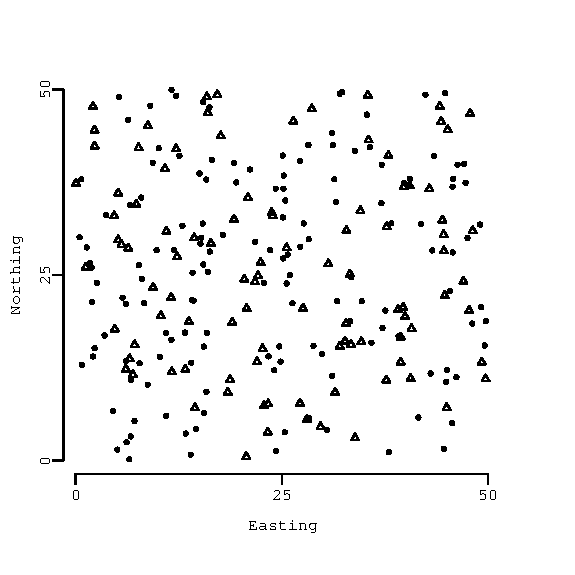
\includegraphics[width=7cm]{synObsa.pdf}}\\
    \subfigure[]{\label{SynObsSurf1}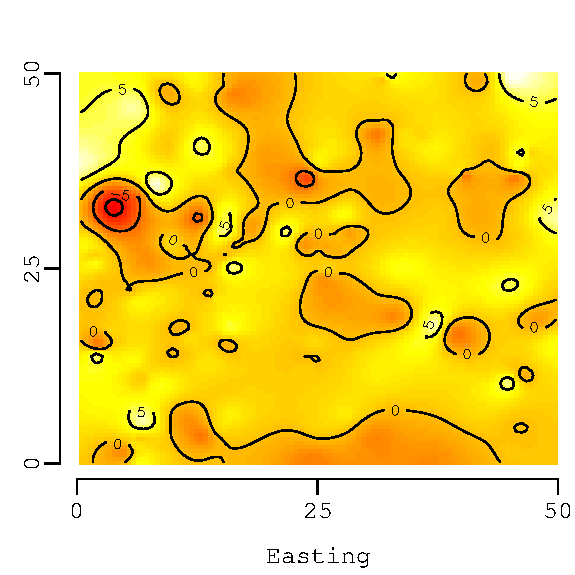
\includegraphics[width=7cm]{synObsb.pdf}}
    \subfigure[]{\label{SynObsSurf2}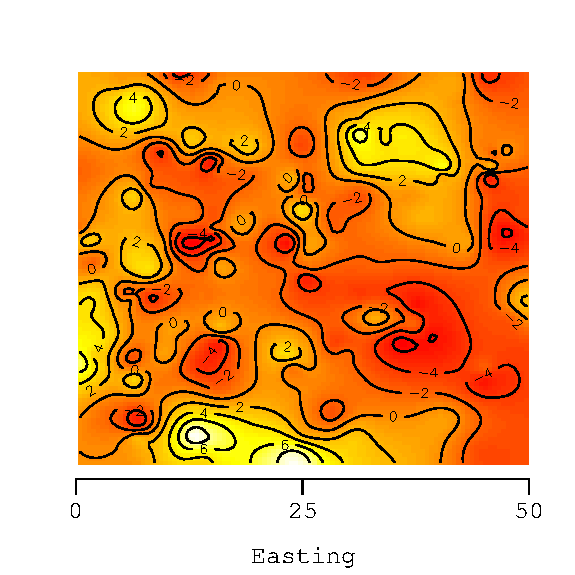
\includegraphics[width=7cm]{synObsc.pdf}} 
  \end{center}
  \caption{(a) Random points used to generate the synthetic data set.  Subsequent parameter estimation is based on 150 ($\bullet$) locations, and prediction at the 100 open triangle locations ($\vartriangle$). Plots (b) and (c) are interpolated surfaces of the first and second response variables, respectivly,  generated with the random points in (a), given parameters, and the marginalized likelihood \ref{marginalizedLikelihood}.}
  \label{Syn}
\end{figure}

\begin{figure}[h!]
\centering
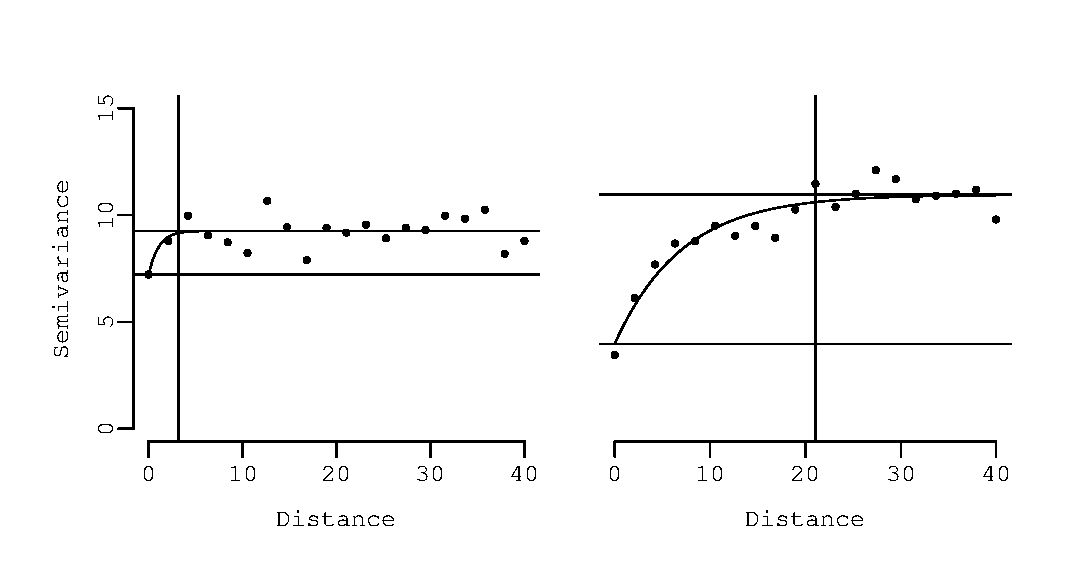
\includegraphics[width=14cm]{synVario.pdf}
\caption{Empirical semivariograms and exponential function REML parameter estimates for the two synthetic response surfaces.  The estimates of the nugget (bottom horizontal line), sill (upper horizontal line), and range (vertical line) for the first surface are approximately 7.2, 9.3, and 3.2 respectively.  The corresponding semivariogram estimates of nugget, sill, and range for the second response surface (right plot)  are 4.0, 11.0, and 21.0, respectively.}
\label{SynObsVario}
\end{figure}
\clearpage
\subsection[Inference and model choice using ggt.sp]{Inference and model choice using \code{ggt.sp}}\label{candidateModels}
The generalized template introduced in Section~\ref{ggt} suggests
several potential models.  Here we consider
seven stationary process models of increasing complexity.  Our focus
is on the alternative specifications of ${\cal A}$ and $\tilde{\bW}$
within (\ref{GeneralDataEquation}).  For each model, we assume an
isotropic spatial process that can be modeled with the exponential
correlation function.

A simple linear regression model (no random effects) is 
\[
\text{Model~1: } {\cal A}\tilde{\bW}=\bzero.
\]
This model would suffice in the presence of negligible
extraneous variation beyond what is explained by the model's
regressors. However, if autocorrelation is seen in each response variable's
surface, as in Figure \ref{Syn}, and the regressors do not
account for this association as a function of distance between
locations, then this model violates the implicit assumption of
conditionally independent observations.

The next four spatial models impose separable association
structures as in (\ref{StationaryDispersionEqn2}). For each model,
$\Sigma_{\tilde{\bW}}=[\tilde{\bK}(\bs_i-\bs_j;\bphi)]_{i,j=1}^{n}$,
$\bphi = \left\lbrace \phi \right\rbrace_{k=1}^{m}$ implies the
response variables share a common spatial decay parameter.  The
first, and simplest, of these models assumes common spatial variance
(i.e., $\sigma^2$) and no non--spatial variance,
\[
\text{Model~2: } \bA=\sigma I_{m}\text{ and } \Psi = \bzero.
\]
The second spatial model allows for a common pure error variance
term (i.e., $\tau^2$),
\[
\text{Model~3: } \bA=\sigma I_{m} \text{ and } \Psi = \tau^2I_m.
\]
The next model extends Model 3 to allow response specific spatial
and pure error variance terms,
\[
\text{Model~4: } \bA=Diag[\sigma_i]_{i=1}^{m}\text{ and } \Psi =
Diag[\tau^2_i]_{i=1}^{m}.
\]
Where Model 4 assumes independence among the response surfaces'
spatial variance, Model 5 explicitly models the off--diagonal
element in the cross--covariance matrix $\bK$,
\[
\text{Model~5: } \bA\text{ and }  \Psi = Diag[\tau^2_i]_{i=1}^{m}
\]
where, recall, $\bA$ is the square root of the $m\times m$
cross--covariance matrix.  The sixth model is the non--separable
form of Model 5, allowing response specific spatial range terms,
\[
\text{Model~6: } \bA, \Psi = Diag[\tau^2_i]_{i=1}^{m}, \text{ and }
\bphi = \left\lbrace \phi_k \right\rbrace_{k=1}^{m}
\]
The final candidate model, extends the diagonal pure error
cross--covariance matrix in Model 6 to a full matrix, allowing for
non--spatial variance dependence among the response surfaces,
\[
\text{Model~7: } \bA, \Psi, \text{ and } \bphi = \left\lbrace \phi_k
\right\rbrace_{k=1}^{m}.
\]

The \code{ggt.sp} function within \pkg{spBayes} was used to fit each
candidate model to the synthetic data.  Following the methods
described in Section \ref{estparams}, the \code{ggt.sp} function
generates samples from each parameter's posterior distribution.
The following code blocks detail the \code{ggt.sp} arguments used to fit
Model 6; the other candidate models can be fit using variations on
these specifications.

The arguments for the \code{ggt.sp} function follow a logical
progression through a Bayesian modeling process.  The initial step
is to assign appropriate prior distributions to each parameter.  The
prior distributions used in \code{ggt.sp} are consistent with
definitions found in Appendix A of Gelman et al. (2004).   The variance
parameters in Model 6 are a $m\times m$ spatial cross-covariance
matrix $\bK$, diagonal non--spatial cross--covariance matrix $\Psi$,
and $m$ spatial range parameters $\bphi$.  The code block below
specifies an inverse--Wishart prior for $\bK$, separate
inverse--Gamma priors for the diagonal elements of $\Psi$, and a
single uniform prior which will be used for both of the $\phi$.  The
empirical semivariograms (Figure \ref{SynObsVario}) were used to
help define the priors' hyperparameters.  For instance, the
semivariograms suggest partial sills of about 3 and 6 for the two
conditional response surfaces (i.e., conditional on the regressors),
and therefore these values serve as the diagonal elements in the
$m\times m$ shape hyperparameter of the  inverse--Wishart prior used
for $\bK$.  The nugget estimates from the semivariograms can guide
the choice of the inverse--Gamma scale hyperparameters (i.e., 7 and
5, respectively).  A shape of 2 in the inverse--Gamma suggests a
distribution with infinite variance centered on the scale
hyperparameter.  An alternative to the inverse--Gamma is the
half--Cauchy also available in \pkg{spBayes} (see Gelman, 2006 for further discussion).  The
\code{LOGUNIF} prior on $\bphi$ indicates a uniform distribution
with support strictly greater than zero.  As noted at the end of
Section \ref{SyntheticData}, $\sim 3/\phi$ can be considered the
effective spatial range.  Therefore, a vague prior on $\bphi$ is a
uniform distribution with support on the interval ($3/3$, $3/0.06$) or (1, 50)
distance units.
 \begin{verbatim}
K.prior <- prior(dist="IWISH", df=2, S=diag(c(3, 6)))
Psi.prior.1 <- prior(dist="IG", shape=2, scale=7)
Psi.prior.2 <- prior(dist="IG", shape=2, scale=5)
phi.prior <- prior(dist="LOGUNIF", a=0.06, b=3)
 \end{verbatim}

The next portion of code describes how each variance parameter is
updated, the assigned prior, starting values, and the order in which
blocks of parameters are updated.  The variance parameters within
the proposed model template are updated with the
Metropolis--Hastings algorithm.  This algorithm requires a
\emph{tuning} or \emph{step--size} value which defines the variance
term in the multivariate normal proposal density.  A tuning value or matrix of the
appropriate dimension must be assigned to each variance parameter.
If a matrix tuning value is specified, it must be invertible. Within
the \proglang{R} list data structure below, the element tags (e.g.,
\code{K}, \code{Psi}, \code{phi}, and if the Mat\'{e}rn
correlation function is used, \code{nu}) are keywords used by \code{ggt.sp} to
link the directives with the given model parameter. Below, for
example, the identity matrix serves as the starting value for $\bK$.
Only three elements need to be updated in the symmetric $\bK$
matrix; therefore, the tuning matrix is $3\times 3$ with diagonal
elements assigned to $\bK$'s lower--triangle column major
elements (i.e., the tuning values are $\bK_{1,1} = 0.1$, $\bK_{2,1}
= 0.5$, $\bK_{2,2} = 0.1$).

Updating parameters in blocks often provides finer control on
Metropolis--Hastings acceptance rate. The value assigned to the
\code{sample.order} list tag controls the block update sequence. The
code below describes a sequential Metropolis--Hastings sampling
scheme that first accepts/rejects the proposed $\bK$ given the
currently accepted $\Psi$ and $\bphi$ samples, then accepts/rejects
$\Psi$ given the currently accepted $\bK$ and $\bphi$, then
accepts/rejects $\bphi$ given the currently accepted $\bK$ and
$\Psi$.
 \begin{verbatim}
var.update.control <-
   list("K"=list(sample.order=0, starting=diag(1, 2),
          tuning=diag(c(0.1, 0.5, 0.1)), prior=K.prior),

        "Psi"=list(sample.order=1, starting=1,
          tuning=0.3, prior=list(Psi.prior.1, Psi.prior.2)),

        "phi"=list(sample.order=2, starting=0.5,
          tuning=0.5, prior=list(phi.prior, phi.prior))
        )
 \end{verbatim}
In the \code{var.update.control} list, the data structure assigned
to the \code{prior} tags determines several model characteristics.
Model 6 is non--separable; therefore, the \code{prior} list within
the \code{phi} tag defines two priors, corresponding to the first
and second spatial process.  If, as in the \code{phi} and \code{Psi}
lists above, multiple priors are defined, the \code{starting} and
\code{tuning} values are recycled.  Alternatively, starting value
and tuning vectors can be passed in place of the scalars.

The regression parameters, $\bbeta$, also receive a prior and update
method.  Unlike the variance parameters, the $\bbeta$ are updated
using either Gibbs (\ref{GibbsBeta}) or Metropolis--Hastings.  The
code below specifies a flat prior with Gibbs updating for each
element in the $\bbeta$ parameter vector.
\begin{verbatim}
beta.control <- list(update="GIBBS", prior=prior(dist="FLAT"))
\end{verbatim}

The last argument that is passed to \code{ggt.sp} defines the number
of posterior samples to collect and, if random spatial
effects, ${\cal A}\tilde{\bW}$, should be recovered.
\begin{verbatim}
run.control <-
  list("n.samples"=5000, "sp.effects"=TRUE)
\end{verbatim}

These arguments are then passed to \code{ggt.sp} along with additional model specifications and data as given in the code below.
\begin{verbatim}
ggt.Model.6 <- ggt.sp(formula=list(Y.1~1, Y.2~1),
                      run.control=run.control,
                      coords=coords,
                      var.update.control=var.update.control,
                      beta.update.control=beta.control,
                      cov.model="exponential")
\end{verbatim}
Specifically, the \code{ggt.sp} call includes: a list of $m$
symbolic model statements\\ \code{formula=list(Y.1$\sim$1,
Y.2$\sim$1)} along with an optional \code{data} argument similar to
\proglang{R}'s \code{lm()} function; a \code{coords} argument which
specifies the $n\times 2$ matrix of observation coordinates; and the
covariance model, \code{cov.model}, to be used (i.e.,
\code{exponential}, \code{matern}, \code{spherical}, or
\code{gaussian}).  The return object, \code{ggt.Model.6} includes
posterior samples for each parameter and random spatial effect samples.

Finally, as described in Section \ref{modFit}, a call to \code{sp.DIC} provides both the marginalized and unmarginalized DIC for the given \code{ggt.sp} return object.  The code below calculates DIC over the interval of 1,000 to 5,000 samples.  The \code{sp.DIC} function also accepts \code{thin} and \code{end} to control the sample interval over which DIC is calculated.
\begin{verbatim}
sp.DIC(ggt.Model.6, DIC.marg=TRUE, DIC.unmarg=TRUE, start=1000)
\end{verbatim}

\subsection{Synthetic data analysis results}
We fit the seven competing models to the synthetic data. For each of
these models, three MCMC chains were run for 5,000
iterations.  Chain mixing occurred within 1,000 iterations, therefore the remaining 12,000 samples
(4,000$\times$3) were retained for posterior analysis.

DIC was used to select the best candidate model to produce response
specific surfaces of random spatial effects $E[\bW |\; Data]$, and subsequent
predictions $E[\bW^{\ast}\,|\, Data]$ and $E[\bY^{\ast}|\; Data]$.

Table \ref{DIC} provides $p_{D}$ and DIC scores for the candidate models.
As noted in Section \ref{modFit}, lower DIC scores suggest better
model performance; therefore, Models 5, 6, and 7 are preferred. Based on the actual number of parameters, Model 5 is
the most parsimonious of the three.  Separability is the distinction
between Model 5 and 6.  Even though Model 6 gave rise to the data,
it is common that the notoriously ill--defined $\phi$ does not
contribute much to model distinctions in formal model fit
comparisons (e.g., DIC).  Rather, we might look to the interpolated
residual surfaces, empirical semivariograms, and $\bphi$ estimates
to determine if there is an advantage to the non--separable model.
In this case, there is a strong distinction in spatial dependence
trends in Figure \ref{Syn} surfaces and Figure \ref{SynObsVario}, and
between estimates of $\phi_1$ and $\phi_2$ in Table
\ref{SyntheticEsts}.  Following these diagnostics, we select Model 6
over Model 5.  

The remaining choice is between Model 6 and 7.  Unlike Model 6, Model 7 explicitly models the off--diagonal element in $\Psi$.  The unmarginalized DIC score in Table \ref{DIC} suggests that Model 7 might be the best fit. However, the marginalized DIC score for Model 7 does not show an advantage over Model 6.  To better understand the contribution of the off--diagonal elements in $\Psi$ or $\bK$, it is often useful to convert these covariance matrices to the corresponding correlation matrices.  For Model 7, the bounds of the 95\% credible interval about $\Psi$'s off--diagonal correlation element are -0.749 and 0.656, which suggests that the non--spatial correlation between the response surfaces is not significant.  Therefore, Model 7 does not seem to add additional insight or a consistently superior model DIC score over Model 6.

\begin{table}[!h]
\begin{center}
\caption{Synthetic data model comparison using the DIC criterion.  For each model both marginalized and unmarginalized $p_{D}$ and DIC were calculated from three chains of 5,000 samples.}\label{DIC}
\begin{tabular}
[c]{|c|c|c|c|c|c|}%
\hline 
\multicolumn{2}{|c}{} & \multicolumn{2}{|c|}{Marginalized} & \multicolumn{2}{|c|}{Unmarginalized}\\
\hline Model & Parameters & $p_{D}$ & DIC & $p_{D}$ & DIC\\\hline
Model~1 & $\tau^2$                          			&  3.049& 993.013& -- & --\\
Model~2 & $\phi$, $\sigma^2$                        	& 3.520& 987.069& -- & --\\
Model~3 & $\phi$, $\sigma^2$, $\tau^2$              	& 4.515& 979.409&  233.626& 1,643.619 \\
Model~4 & $\phi$, $\sigma^2_m$, $\tau^2_m$	&  5.382& 966.157&  256.186& 1,537.190\\
Model~5 &  $\phi$, $\bA$, $\tau^2_m$			&  6.464& 958.586&  260.640& 1,450.184\\
Model~6 &  $\phi_m$, $\bA$, $\tau^2_m$             &  6.141& 957.195&  236.838& 1,492.053\\
Model~7 &  $\phi_m$, $\bA$, $\Psi$                  	&  5.879& 957.882&  206.663& 1,446.000\\
\hline
\end{tabular}
\end{center}
\end{table}

Under models with $\Psi = \bzero$, for instance Models 1 and 2, the unmarginalized target likelihood reduces to the marginalized likelihood.  Therefore, the unmarginalized DIC and associated statistics are omitted from Table \ref{DIC}. 

Table \ref{SyntheticEsts} provides parameter estimate summaries for
Model 6.  Because the synthetic data is only one realization of the defined model, it would be a rare occurrence for the
\emph{true} parameters to fall outside of the estimated 2.5\%--97.5\% percentiles (i.e., only a 5\% chance).  Indeed, Table \ref{SyntheticEsts} shows that the estimated
intervals cover the corresponding true parameters defined in Section
\ref{SyntheticData}.  Further, converting the estimates for the
cross--covariance matrix $\bK$ to the 50\% (2.5\%, 97.5\%)
percentiles of the posterior cross--correlation matrix, we see that
the off--diagonal element is -0.475 (-0.791, -0.095), again
covering the true negative association between the response surfaces
of -0.707.

\begin{table}[!h]
\begin{center}
\caption{Percentiles of the posterior distributions of the parameters in Model 6.  $\beta$ subscripts refer to the response variable and parameter, respectively.  Subscripts on $\bK$ and $\Psi$ refer to the covariance matrix element.  Subscripts on the spatial range parameters, $\phi$, refer to the response variable. Summaries generated from three chains of 4,000 samples.} \label{SyntheticEsts}
\begin{tabular}
[c]{|c|c|}%
\hline Parameter & Estimates: 50\% (2.5\%, 97.5\%)\\\hline
$\beta_{1,0}$ &  1.086 (0.555, 1.628)\\
$\beta_{2,0}$ &  -0.273 (-1.619, 1.157)\\
\hline
$\bK_{1,1}$ &  1.801 (0.542, 6.949)\\
$\bK_{2,1}$ & -1.784 (-3.604, -0.357)\\
$\bK_{2,2}$ &  8.253 (4.645, 13.221)\\
\hline
$\Psi_{1,1}$ & 7.478 (3.020, 10.276)\\
$\Psi_{2,2}$ & 2.276 (0.832, 5.063)\\
\hline
$\phi_{1}$ & 1.024 (0.243, 2.805)\\
$\phi_{2}$ & 0.193 (0.073, 0.437)\\
\hline
\end{tabular}
\end{center}
\end{table}

Figure \ref{SynWSurf} provides the interpolated surfaces of recovered
random spatial effects $E[\bW |\; Data]$.  Conditioning only on the
models' intercept terms, that are constant across the domain,
causes the mean random effect surfaces to look nearly identical to
the observed surfaces Figure \ref{Syn}.

\begin{figure}[h!]
\centering
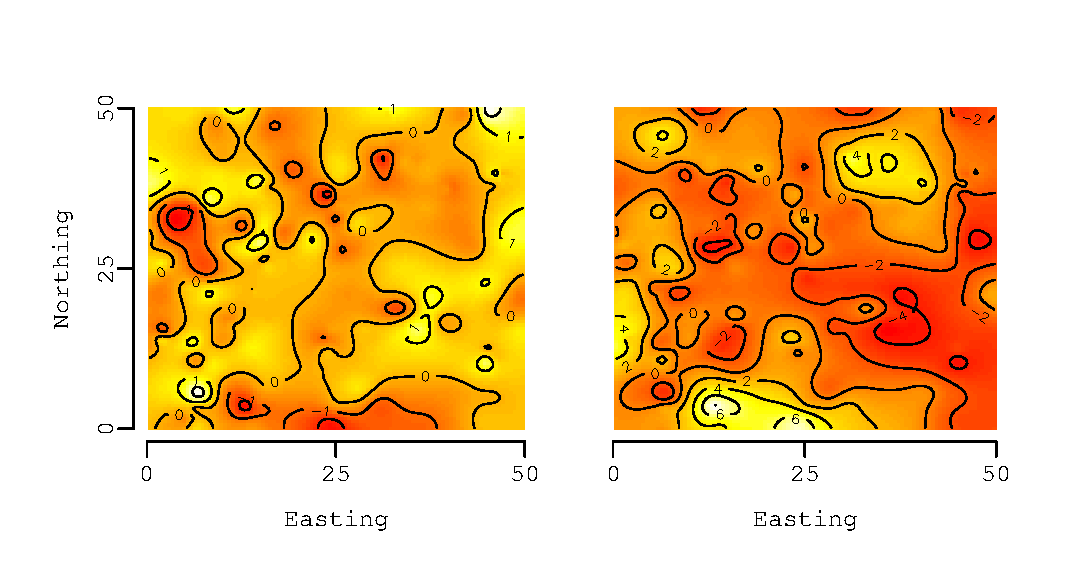
\includegraphics[width=14cm]{synWSurf.pdf}
\caption{Interpolated surfaces of the recovered random spatial effects for Model~6, $E[\bW |\; Data]$.}
\label{SynWSurf}
\end{figure}


\subsection[Prediction using sp.predict]{Prediction using \code{sp.predict}}
The \code{sp.predict} function will predict $\bW^{\ast}$ and
$\bY^{\ast}$ for any set of $n^{\ast}$ new sites, given a
\code{ggt.sp} return object and the coordinates and covariates of
the new sites.  Following the methods detailed in Section
\ref{postPred}, \code{sp.predict} returns samples from the joint
posterior predictive distribution of the set of new sites.  This
process is illustrated using the \code{ggt.sp} return object,
\code{ggt.Model.6}, and the 100 prediction sites in Figure
\ref{SynObs} (i.e., sites denoted by a triangle symbol).  The code
below calls the \code{sp.predict} function. 
\begin{verbatim}
sp.pred <-
  sp.predict(ggt.Model.6, pred.coords=coords, pred.covars=covars)
\end{verbatim}
In the above code, the \code{pred.coords} value is the
$n^{\ast}\times 2$ matrix of new coordinates and \code{pred.covars}
is the $n^{\ast}\times p$ design matrix $\bX^{\ast}$.  This
multivariate design matrix can be created by passing a list of the
$m$ models' design matrices to the \code{mk.mv.X} function provided
in \pkg{spBayes}. The \code{sp.predict} function also accepts \code{start}, \code{thin}, and \code{end} to control the sample interval over which the predictions are calculated.

Figure \ref{SynPredWSurf} provides an interpolated surface generated from each new point's mean predicted random spatial effect, $E[\bW^{\ast}\,|\, Data]$.  Without covariates, prediction relies on the strength of the estimated spatial dependence among observed sites and the intercept term which serves as a constant offset across the domain.  Both predicted surfaces in Figure \ref{SynPredWSurf} show substantial smoothing.  Smoothing is exacerbated as spatial range increases, as seen in the second response surface predictions.  As noted in Table \ref{SyntheticEsts}, neither intercept term is significant; therefore, Figure \ref{SynPredYSurf} appears to be only marginally different than the surface of predicted random effects.

\begin{figure}[h!]
  \begin{center}
    \subfigure[]{\label{SynPredWSurf}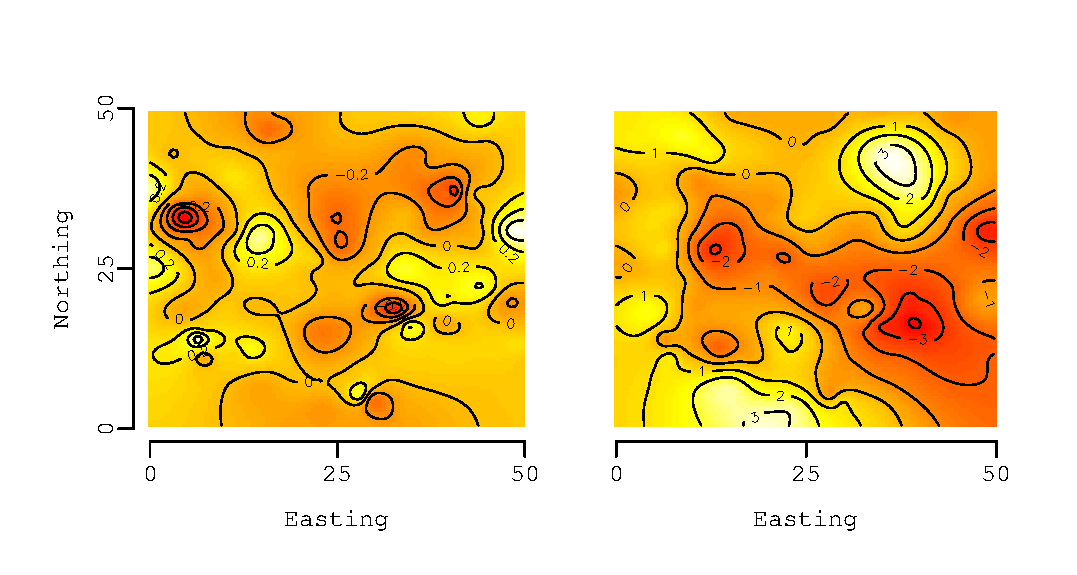
\includegraphics[width=14cm]{synPredWSurf.pdf}}\\
    \subfigure[]{\label{SynPredYSurf}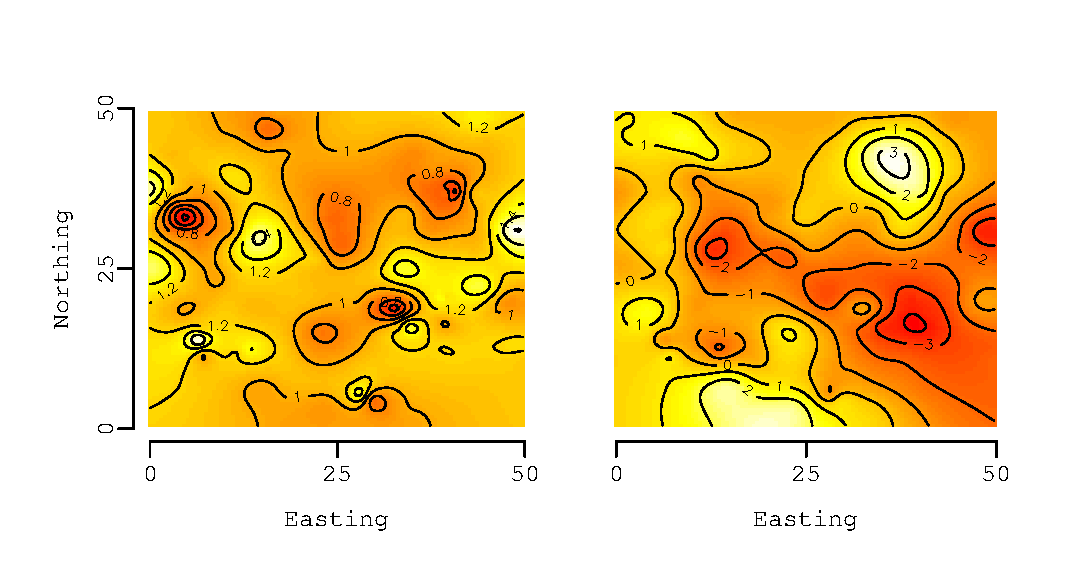
\includegraphics[width=14cm]{synPredYSurf.pdf}} 
  \end{center}
  \caption{(a) Interpolated surfaces of the predicted random spatial effects for Model~6, $E[\bW^{\ast}\,|\, Data]$. (b) Interpolated surfaces of the posterior predictive distributions for Model~6, $E[\bY^{\ast}|\; Data]$.}
  \label{SymPred}
\end{figure}
\clearpage
\subsection{Forest inventory data}\label{RealData}
Maps of forest attributes are important for quantifying forest carbon dynamics, monitoring forest habitat change, forecasting wood availability, and a host of other forest management and environmental initiatives.  The data used in the example below is taken from permanent georeferenced forest inventory plots on the USDA Forest Service Bartlett Experimental Forest (BEF) in Bartlett, New Hampshire.  The 1,053 hectare BEF covers a large elevation gradient from the village of Bartlett in the Saco River valley at 207 meters to about 914 meters above sea level. For this illustration, the focus is on predicting the spatial distribution of basal area and total tree biomass per hectare across the BEF.

Basal area is the cross--sectional area of a tree stem 1.37 meters above the ground and is measured as square meters per hectare.  Tree biomass is measured as the weight of all above ground portions of the tree, expressed here as metric tons per hectare.  Within the data set, basal area (BA) and biomass (BIO) per hectare are recorded at 300 forest inventory plots.  Satellite imagery and other remotely sensed variables have proved useful regressors for predicting these attributes.  One spring 2002 date of 30$\times$30 Landsat 7 ETM+ satellite imagery was acquired for the BEF.  The image was transformed to tasseled cap components of brightness (1), greenness (2), and wetness (3) using data reduction techniques.  The three resulting spectral variables are labeled TC1, TC2, and TC3.  In addition to these spectral variables, digital elevation model data was used to produce a 30$\times$30 elevation (ELEV)  layer for the BEF.  The centroids of the 300 georeferenced inventory plots were intersected with the elevation (ELEV) and spectral variables.

To demonstrate parameter estimation and prediction, we selected randomly 150 inventory plots for model construction and left the remaining 150 for subsequent predictive mapping.  For reference, the 150 model points in Figure~\ref{RealObs} are used to produce an interpolated surface for each of the two response variables, Figures \ref{RealObsSurf1} and \ref{RealObsSurf2}.

\begin{figure}[h!]
  \begin{center}
    \subfigure[]{\label{RealObs}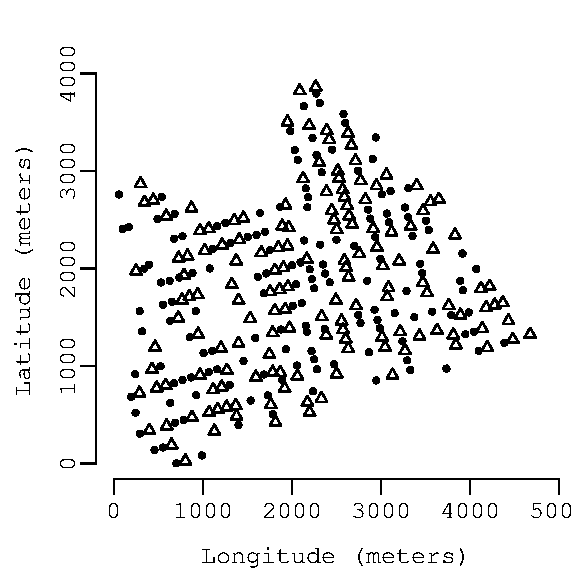
\includegraphics[width=7cm]{befObsa.pdf}}\\
    \subfigure[]{\label{RealObsSurf1}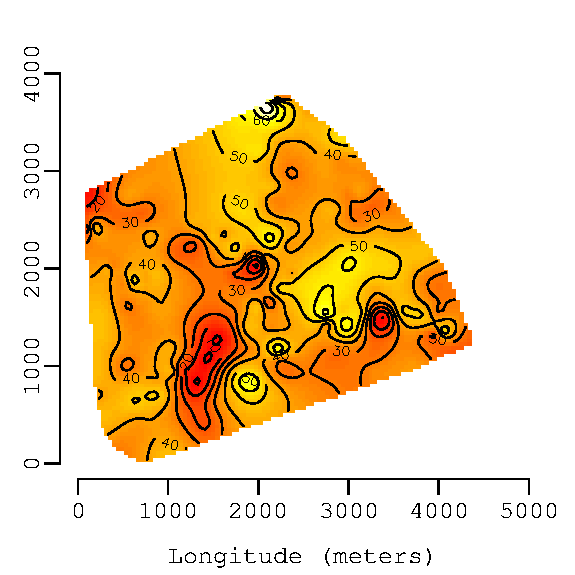
\includegraphics[width=7cm]{befObsb.pdf}}
    \subfigure[]{\label{RealObsSurf2}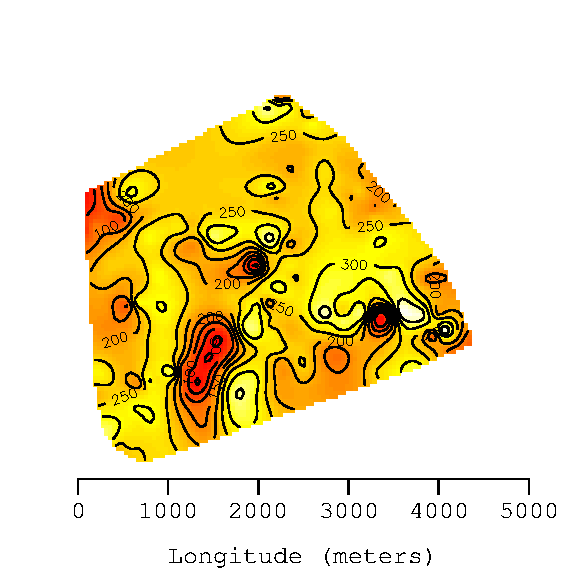
\includegraphics[width=7cm]{befObsc.pdf}} 
  \end{center}
  \caption{(a) Forest inventory plots across the Bartlett Experimental Forest.  The 300 plots were divided randomly into 150 plots used for parameter estimation denoted with solid dot symbols ($\bullet$) and the remaining 150 used for prediction marked with triangle symbols ($\vartriangle$).  Plots (b) and (c) are interpolated surfaces of basal area per hectare and metric tons of biomass per hectare, respectivly.}
  \label{Real}
\end{figure}

Previous results suggest that there is positive spatial and non--spatial association between the conditional response surfaces (i.e., conditional on the regressors).  Further, the univariate empirical semivariograms for the response variables show some disparity between the spatial ranges, specifically, spatial dependence among sites is smaller for measures of basal area per hectare.  Therefore, we fit a non--separable spatial regression with full spatial and non--spatial cross--covariance matrices, $\bK$ and $\Psi$.  Further, we assume that spatial dependence can be modeled with the simple exponential correlation function.  This specification corresponds to Model 7 in Section \ref{candidateModels}.

As in the previous illustration, the univariate empirical semivariograms provide guidance for starting values and prior hyperparameters.  The \code{ggt.sp} directives for one of the six chains used for model parameter estimation are detailed in the code blocks below.  Again, defining priors is the first step in the modeling process.
\begin{verbatim}
K.Psi.prior <- prior(dist="IWISH", df=2, S=matrix(c(100, 0, 0, 2600), 2, 2))
phi.prior <- prior(dist="LOGUNIF", a=0.0015, b=0.03)
\end{verbatim}
The inverse--Wishart prior is used for both cross--covariance matrices.  The empirical semivariograms suggest that the nugget and partial sill are about equal for each response variable (i.e., $\sim100$ for basal area and $\sim2600$ for biomass).  The vague scale matrix defined for the common inverse--Wishart centers each response on the suggested values but does not impose any off--diagonal association.  The noninformative prior on the spatial range parameters corresponds to an interval of 100 to 2,000 meters.

The following code block defines the starting values of $\bK^{1/2}$ and $\Psi^{1/2}$; Metropolis--Hastings tuning values; update method for the $\bbeta$; the number of samples to take; and the regression model for each response surface.

\begin{verbatim}
K.Psi.starting <- matrix(c(10, 80, 0, 10), 2, 2)

var.update.control <-
  list("K"=list(sample.order=0, starting=K.Psi.starting,
         tuning=diag(c(0.15, 1.75, 0.15)), prior=K.Psi.prior),
       "Psi"=list(sample.order=1, starting=K.Psi.starting,
         tuning=diag(c(0.15, 1.75, 0.15)), prior=K.Psi.prior),
       "phi"=list(sample.order=2, starting=0.006,
         tuning=0.5, prior=list(phi.prior, phi.prior)))

beta.control <- list(update="GIBBS", prior=prior(dist="FLAT"))

run.control <- list("n.samples"=10000, "sp.effects"=TRUE)

resp.1 <- BA~ELEV+TC1+TC2+TC3
resp.2 <- BIO~ELEV+TC1+TC2+TC3
\end{verbatim}

Finally these directives are passed to the \code{ggt.sp} function along with additional arguments which define the model plot coordinates and the desired spatial correlation function.
\begin{verbatim}
ggt.chain.1 <-
  ggt.sp(formula=c(resp.1, resp.2), run.control=run.control,
         coords=coords, var.update.control=var.update.control,
         beta.update.control=beta.control,
         cov.model="exponential")
\end{verbatim}

\subsection{Forest inventory data analysis results}
For parameters estimation, six MCMC chains were run for 10,000 iterations.  The six chains allowed for dispersed parameter starting values and because we are interested in the influence of the prior specification on parameter estimates, each chain received a different inverse--Wishart hyperparameter scale matrix.  As seen in the synthetic data set analysis, chain mixing occurred within 1,000 iterations.  Therefore, 54,000 samples were retained for posterior analysis.  Visual interpretation of the changes and resulting parameter estimates suggest that for this data set, the inverse--Wishart scale hyperparamter has negligible influence on chain convergence.

Table \ref{RealEsts} provides the credible intervals for each parameter in the model.  These intervals show that several regressors help explain the variation in both basal area and biomass per hectare.  The significance of the off--diagonal elements $\bK_{2,1}$ and $\Psi_{2,1}$ suggests that there is positive spatial and non--spatial association between the conditional response surfaces.  Additional insight is gained by converting these off--diagonal covariances to correlations, specifically 0.886 (0.241, 0.952) and 0.84 (0.111, 0.941) are the 50\% (2.5\%, 97.5\%) percentiles of the $\bK_{2,1}$ and $\Psi_{2,1}$ elements, respectively.  The spatial range estimates in Table \ref{RealEsts} do not support a distinction between the responses' spatial dependence structure, therefore, the separable form of this model might be considered.

\begin{table}[h!]
\begin{center}
\caption{Percentiles of the posterior distribution of model parameters.  $\beta$ subscripts refer to the response variable and parameter, respectively.  Subscripts on $\bK$ and $\Psi$ refer to the covariance matrix element.  Subscripts on the spatial range parameters, $\phi$, refer to the response variable model. Summaries generated from six chains of 9,000 samples.} \label{RealEsts}
\begin{tabular}
[c]{|c|c|}%
\hline Parameter & Estimates: 50\% (2.5\%, 97.5\%)\\\hline
$\beta_{1,0}$ &  -66.912 (-147.658, 14.279)\\
$\beta_{1,ELEV}$ & -0.011 (-0.030, 0.007) \\
$\beta_{1,TC1}$ &  1.287 (0.366, 2.184)\\
$\beta_{1,TC2}$ &  -1.051 (-1.638, -0.419)\\
$\beta_{1,TC3}$ &  1.502 (0.690, 2.293)\\
$\beta_{2,0}$ &  -312.771 (-838.557, 207.984)\\
$\beta_{2,ELEV}$ &  -0.076 (-0.198, 0.041)\\
$\beta_{2,TC1}$ &  6.899 (1.072, 12.701)\\
$\beta_{2,TC2}$ &  -4.063 (-7.835, -0.083)\\
$\beta_{2,TC3}$ &  6.036 (0.884, 11.141)\\
\hline
$\bK_{1,1}$ &  85.346 (14.806, 152.670)\\
$\bK_{2,1}$ & 519.223 (20.078, 930.767)\\
$\bK_{2,2}$ &  3920.109 (316.533, 6863.146)\\
\hline
$\Psi_{1,1}$ & 71.814 (13.653, 142.901)\\
$\Psi_{2,1}$ & 359.778 (11.178, 838.964)\\
$\Psi_{2,2}$ & 2686.357 (415.428, 5916.541)\\
\hline
$\phi_{1}$ & 0.013 (0.003, 0.029)\\
$\phi_{2}$ & 0.017 (0.005, 0.029)\\
\hline
\end{tabular}

\end{center}
\end{table}

Given the parameters posterior samples, we can now turn to predicting basal area and biomass for the holdout set of sites marked with triangle symbols in Figure \ref{RealObs}.  Alternatively, we could make predictions for each $30\times 30$ meter pixel in the image stack of derived satellite spectral components and ELEV variable.  Again, the predictions are made using the \code{sp.predict} function and passing in the \code{ggt.chain.1} object returned from \code{ggt.sp} along with the new sites' coordinates and covariates.
\begin{verbatim}
BA.X <- cbind(rep(1, 150), ELEV, TC1, TC2, TC3)
BIO.X <- cbind(rep(1, 150), ELEV, TC1, TC2, TC3)

pred.covars <- mk.mv.X(list(BA.X, BIO.X))

sp.pred <- sp.predict(ggt.chain.1, start=5000, thin=5,
                      pred.coords=coords,
                      pred.covars=covars)
\end{verbatim}
The \code{sp.pred} object contains the posterior predictive samples for $\bW^{\ast}$ and $\bY^{\ast}$.  These samples were used to produce the point estimate surfaces in Figure \ref{RealPred}.  Additionally, we could map some function of the posterior samples.  For example, we might map the range between the upper and lower 95\% credible interval of $\bY^{\ast}$ to understand how uncertainty in prediction varies across the domain.

\begin{figure}[htp]
  \begin{center}
    \subfigure[]{\label{RealPredWSurf}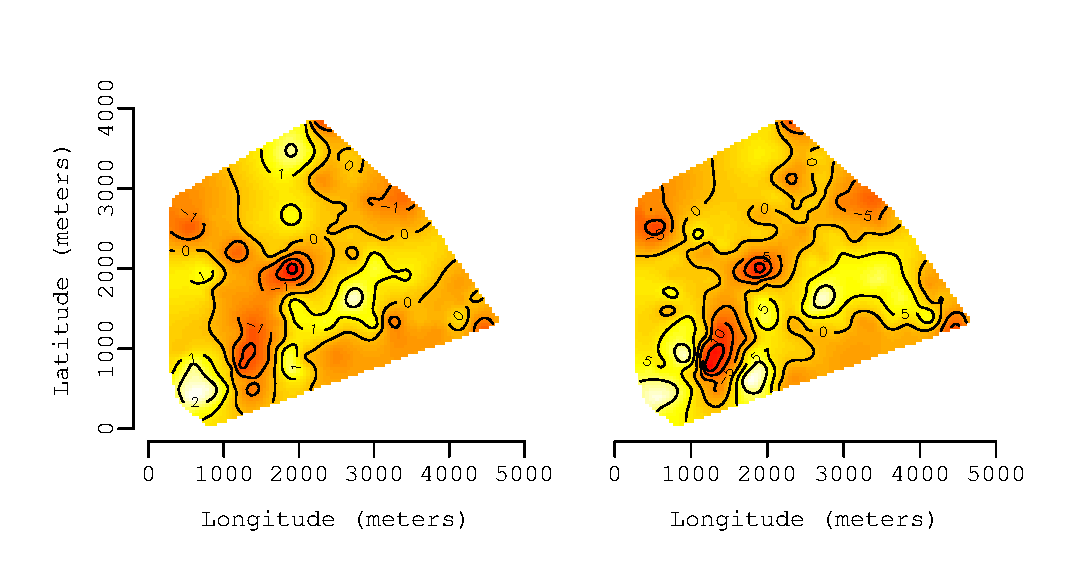
\includegraphics[width=14cm]{befPredWSurf.pdf}}\\
    \subfigure[]{\label{RealPredYSurf}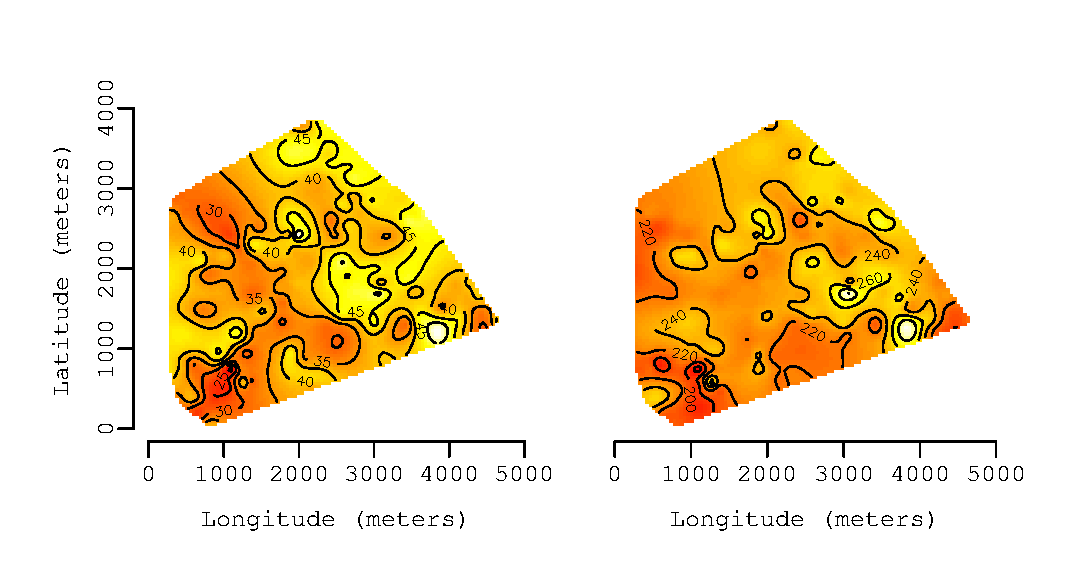
\includegraphics[width=14cm]{befPredYSurf.pdf}} 
  \end{center}
  \caption{(a) Interpolated surfaces of the predicted random spatial effects for basal area per hectare (left plot) and metric tons of biomass per hectare (right plot), $E[\bW^{\ast}\,|\, Data]$. (b) Interpolated surfaces of the posterior predictive distributions for basal area per hectare (left plot) and metric tons of biomass per hectare (right plot), $E[\bY^{\ast}|\; Data]$.}
  \label{RealPred}
\end{figure}
\clearpage
\section{Summary}\label{Summary}
There is a need within the scientific community for software tools capable of efficiently fitting complex co--varying point level Gaussian spatial process models.  The generalized template introduced in Section~\ref{ggt} allows univariate and multivariate Gaussian models to be cast in a common framework.  This facilitates model parameter estimation and predictive inference implemented in the \pkg{spBayes} package.  As detailed in the formal \pkg{spBayes} documentation, the \code{ggt.sp} functions accepts the set of usual covariance functions for modeling spatial dependence, and prior distributions for the variance and covariate parameters.

Although the illustrations presented here consider only bivariate processes, \code{ggt.sp} and the support functions easily accommodate any number of response variables and associated covariates.  Computing time is the only restriction.  The computational burden for implementing our template will explode with a large number of locations. This is known as the so--called ``big--N'' problem in spatial statistics and is an area of active research. Strategies for addressing this problem involve representing the spatial process $\bW(\bs)$ over a smaller set of representative locations (called knots).

We hope future releases of \pkg{spBayes} will continue to help fulfill multivariate spatial process modeling needs.  In the near-term, we plan to include facilities for modeling big-N problems, spatially varying regressors, multi--resolution or spatially nested models, and non-Gaussian response models.

\section{References}

\begin{description}
\item Banerjee, S., Carlin, B.P., and Gelfand, A.E. (2004). \emph{Hierarchical Modeling and Analysis for Spatial Data}. Boca Raton, FL: Chapman and Hall/CRC Press.

\item Carlin, B.P., and Louis, T.A. (2000). \emph{Bayes and empirical Bayes methods for data analysis}. Boca Raton, Florida: Chapman and Hall.

\item Chil\'es, J.P., and Delfiner, P. (1999). \emph{Geostatistics: Modelling Spatial Uncertainty}. New York: John Wiley and Sons.

\item Cressie, N.A.C. (1993). \emph{Statistics for Spatial Data}, 2nd ed. New York: Wiley.

\item Gelman A. (2006). Prior distributions for variance parameters in hierarchical models. \emph{Bayesian Analysis}, 3, 515–533.

\item Gelman, A., Carlin, J.B., Stern, H.S., and Rubin, D.B. (2004). \emph{Bayesian Data Analysis}. 2nd ed. Boca Raton, FL: Chapman and Hall/CRC Press.

\item Gilks, W., Richardson, S., and Spiegelhalter, D. (1996). \emph{Markov Chain Monte Carlo in Practice}. Boca Raton: Chapman and Hall/CRC.

\item Harville, D.A. (1997). \emph{Matrix Algebra from a Statistician's Perspective}. New York: Springer.

\item Majumdar, A., and Gelfand, A.E. (2006). Spatial Modeling for Multivariate Environmental Data Using Convolved Covariance Functions. Technical Report Institute of Statistics and Decision Sciences, Duke University, Durham, NC.

\item M{\o}ller, J. (2003). \emph{Spatial Statistics and Computational Method}. New York: Springer.

\item Ribeiro Jr., P.J., and Diggle, P.J.(2001). geoR: A Package for Geostatistical Analysis. R News, 1(2), 14–18.

\item Schabenberger, O., and Gotway, C.A. (2004). \emph{Statistical Methods for Spatial Data Analysis (Texts in Statistical Science Series)}. Boca Raton: Chapman and Hall/CRC.

\item Spiegelhalter, D.J., Best, N.G., Carlin, B.P., and van der Linde, A. (2002). Bayesian measures of model complexity and fit (with discussion and rejoinder). \emph{Journal of the Royal Statistical Society, Series B}, 64, 583--639.

\item Stein, M.L. (1999). \emph{Interpolation of Spatial Data: some theory for kriging}. New York: Springer.

\item Wackernagel, H. (2003). \emph{Multivariate Geostatistics: An Introduction with Applications}. 3rd ed. Berlin: Springer-Verlag.
\end{description}

\end{document}
